After successful calibration, cameras are integrated to mobile robot. This chapter starts with an introduction of mobile robot used in the thesis. It explains the procedure adopted for base frame transformations of all sensors. Furthermore, proposed implementation, data acquisition process and different experiment data sets taken for evaluation are covered.

\section{Setup}
The mobile platform used for this scope of work is TurtleBot2e \cite{turtlebot2}, a 2nd generation robot of turtlebots family also known as Kobuki. The robot is equipped with SICK 2D \acrshort{lidar} TIM571 \cite{sick}, SICK Picocam and Genius-Widecam (F100) as shown in figure \ref{fig:turtlebot}.
\begin{figure}[h!]
	\centering
	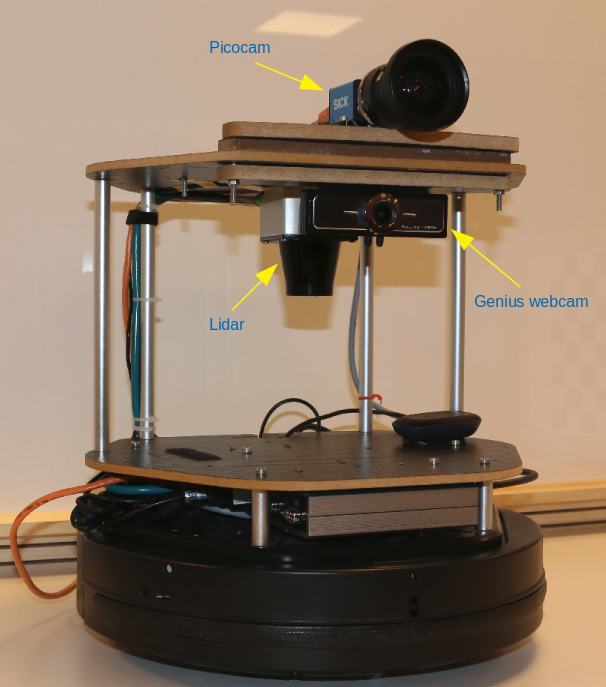
\includegraphics[width=0.62\textwidth]{turtlebot}
	\caption{Turtlebot equipped with \acrshort{lidar}, picocam, genius widecam}
	\label{fig:turtlebot}
\end{figure}
\subsection{Base frame transformation}
In order to compare the odometry results from all three sensors a common base is required. Therefore, base-frame transformations is done with respect to \acrshort{lidar} center as reference frame. A 2D chessboard placed at fixed distance of 1000 mm from \acrshort{lidar} is used as target. OpenCV software \cite{opencvcalib} is used to calculate extrinsic parameters (rotation and translation) with respect to chessboard as base frame. These parameters are further transformed to \acrshort{lidar} considering it as base-frame. An illustration of procedure is given in figure \ref{fig:transformation}.
\begin{figure}[H]
	\centering
	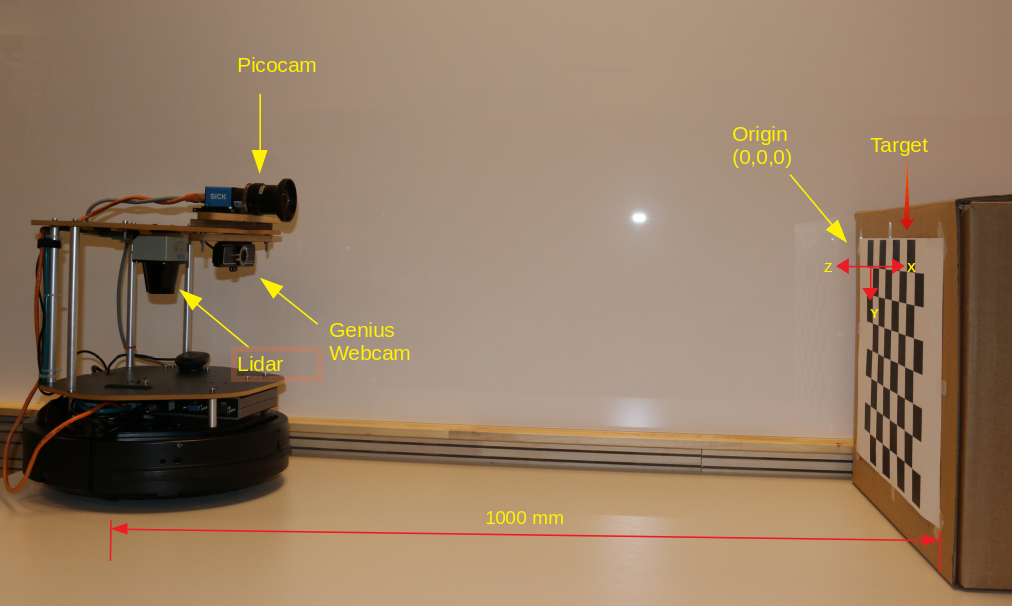
\includegraphics[width=1.0\textwidth]{frame_transformation}
	\caption{Setup to compute base-frame transformation}
	\label{fig:transformation}
\end{figure}
\noindent The distance between \acrshort{lidar} to chessboard target is confirmed with help of SICK mapping tool as shown in figure \ref{fig:smet}. \acrshort{lidar} center is determined using figure \ref{fig:tim} marked as 5 (light transmitter).
\begin{figure}[H]
	\centering
	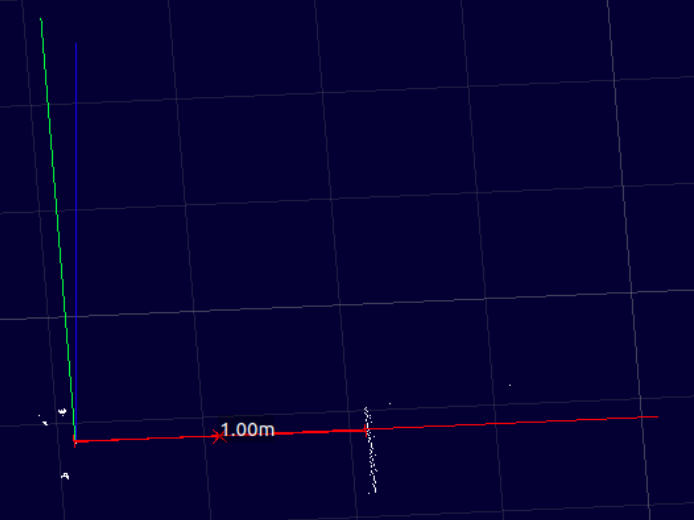
\includegraphics[width=0.7\textwidth]{smet}
	\caption{Distance measured between \acrshort{lidar} and target using SICK mapping tool}
	\label{fig:smet}
\end{figure}
\begin{figure}[H]
	\centering
	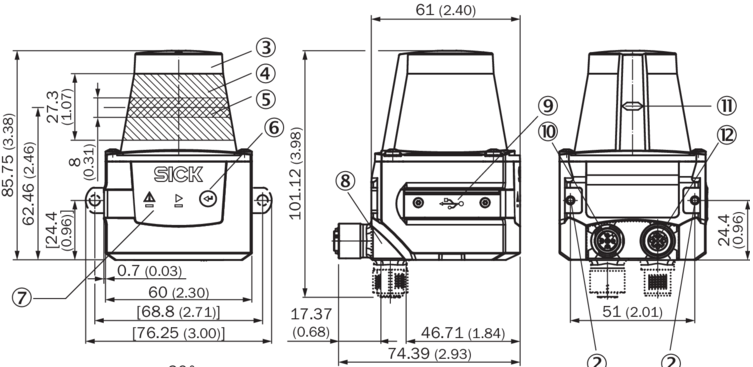
\includegraphics[width=1.0\textwidth]{TIM571}
	\caption{Front view of dimensional drawing of \acrshort{lidar} TIM571 used in this thesis \cite{sick}}
	\label{fig:tim}
\end{figure}
\noindent Equation \ref{eq:trans} explains transformations between chessboard target origin, \acrshort{lidar} and camera. The result is given in \ref{section:A.3}.
\begin{equation*}
\label{eq:trans}
  ^{cam}T_{lidar}  = ^{cam}T_{traget} * ^{target}T_{lidar} 
\end{equation*} 
where $ ^{i}T_{j} $ is transformation matrix (R,t) of i with respect to j in homogeneous coordinates ($ \mathbb{R}^{4} $).

\section{Software Implementation}
Software implementation of all three algorithms for both cameras and \acrshort{lidar} odometry is shown in figure \ref{fig:implementation}. For every experiment three types of raw data are acquired in form of stream container. The driver workers for each sensor convert this data in to useful format. Figure \ref{fig:implementation} shows how raw data is processed to algorithm compatible form and feed as an input to respective algorithm. The output of all odometry algorithms is in from of position and orientation of the sensors at every timestamp and then transformed to the base frame which is \acrshort{lidar} origin. The resulting vehicle pose is also saved in a .text file in order to evaluate results.
\begin{figure}[H]
	\centering
	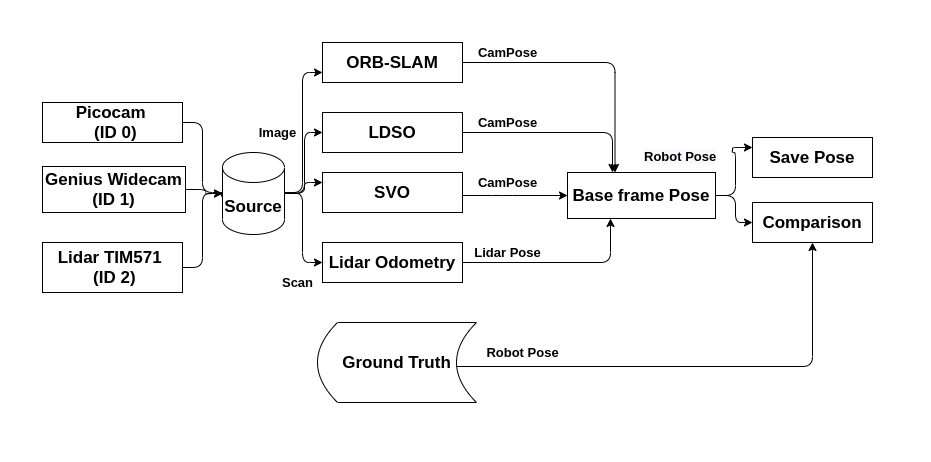
\includegraphics[width=1.0\textwidth]{implementation}
	\caption{Software implementation structure of \acrshort{vo} algorithms for the purpose of comparison}
	\label{fig:implementation}
\end{figure}

\section{Data Acquisition}
Data acquisition step depends on some criteria like the use cases, environment etc. In this thesis scope the use case is warehouse applications in indoor environment. A typical warehouse scenario used in this thesis can be seen in figure \ref{fig:warehouse}. Furthermore, \acrshort{vo} can not perform well in dynamic environment so the surrounding is also static with no human activity. As direct methods track image intensities and assume constant brightness, tests are taken using artificial lighting in indoor environment with no frequent brightness changes.
\begin{figure}[H]
	\centering
	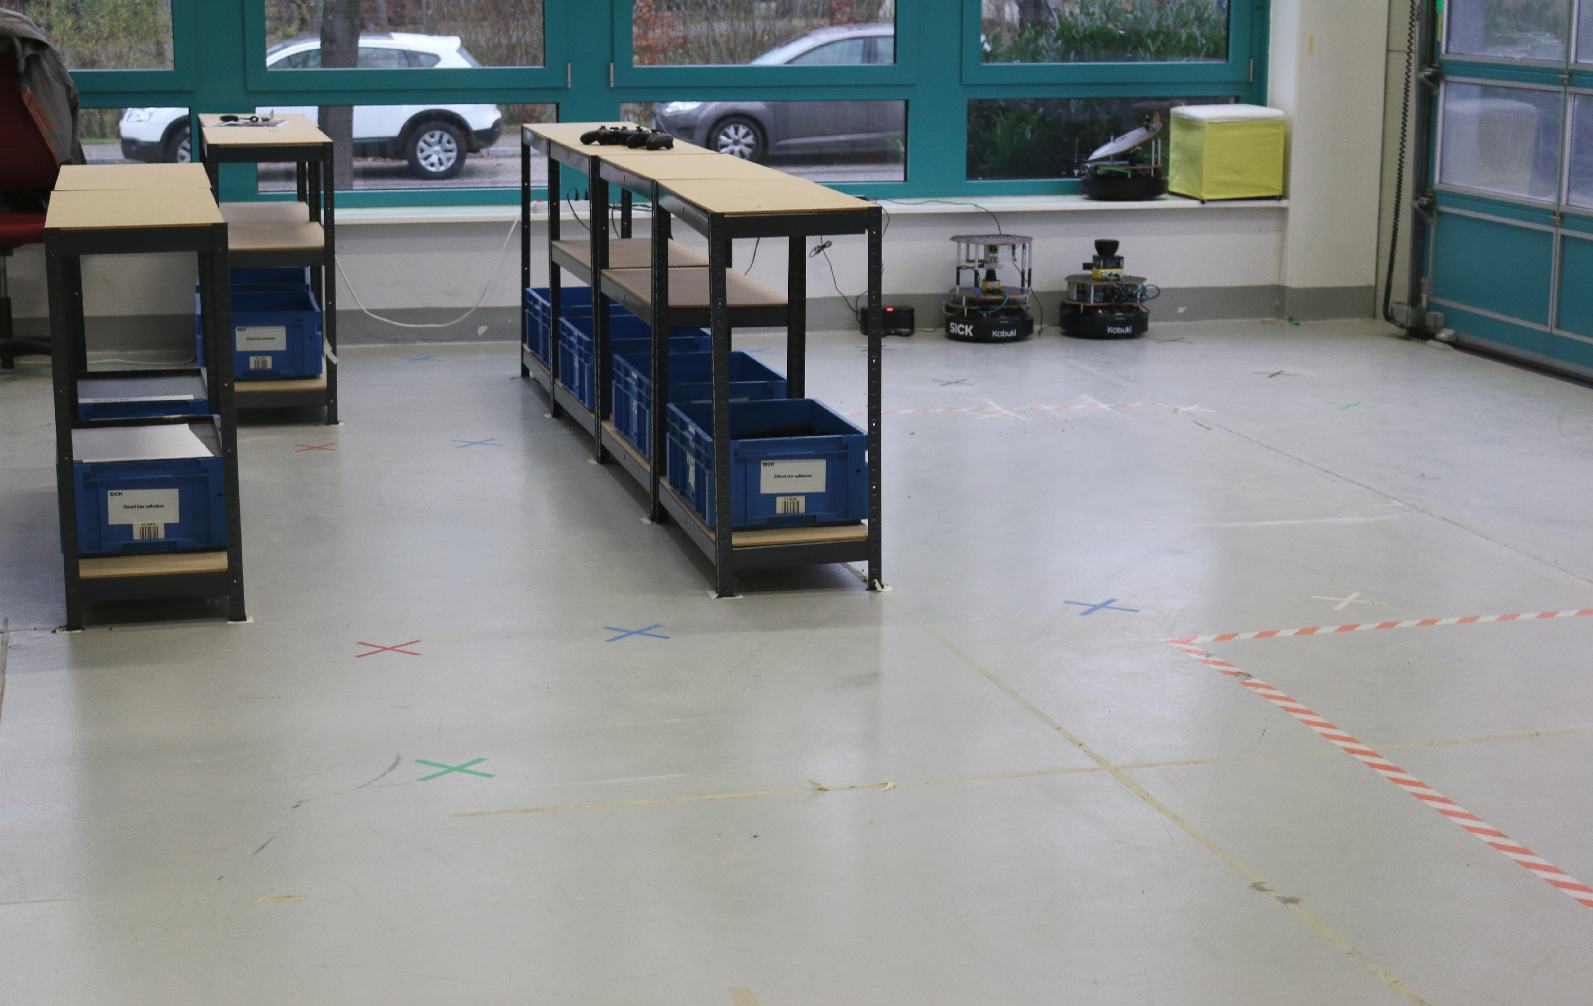
\includegraphics[width=0.8\textwidth]{warehouse}
	\caption{A warehouse scenario used in \acrshort{vo} experiment}
	\label{fig:warehouse}
\end{figure}
\noindent Real-time implementation is not done due to evaluation purpose of all algorithms. Therefore, all tests are first recorded and then evaluated in offline mode on a 16GB Ubuntu-18.04 PC. Every measurement includes the recording of Picocam, Genius Widecam F100 and \acrshort{lidar} TIM571 in form of .sc file. Mobile robot is operated manually with Xbox 360 Wireless Bluetooth controller. Camera resolution for Picocam is $ 1024 * 1024 $ and for Genius Widecam F100 is $ 1280 * 720 $. Exposure time for Picocam is set to 20 milliseconds and \acrshort{fps} for Picocam is 17 and for Genius Widecam it is 30. A Docker image is created for the measurements. The details of various types of recording taken during experiment is shown in table \ref{table:recording}.
\begin{table}[H]
	\centering
	\renewcommand{\arraystretch}{1.5}
	\begin{tabular}{ l l  l  l  p{5cm} }
		
		\textbf{Number} & \textbf{Date} & \textbf{Pattern}  & \textbf{Length}  & \textbf{Notes}  \\    
		\hline
		1 & 18.12.2020 &  Straight  & 30 s & path length $\sim$16 m  \\ 
		\hline
		2 & 14.12.2020  & Rectangle & 1 min 13 s   & length $\sim$8 m, width $\sim$2 m, No loop\\ 
		\hline
		3 & 11.11.2020  & Repeated  & 1 min 27 s  & 1 loop with same origin and end point\\ 
		\hline
		4 & 03.11.2020   & Multi loop  &  3 min 35 s  & No \acrshort{lidar} data recorded \\
		\hline
		5 & 18.12.2020 & Eight (8) & 1 min 24 s &  1 loop, mostly rotation  \\
		\hline
	\end{tabular}
	\caption{Details of data recorded during the experiment}
	\label{table:recording}
\end{table}

\section{Improvements}
This section describes some modifications done in original algorithms to get the best performance and result. The experiments are evaluated after these improvements. 

\subsection{\acrshort{orb}-\acrshort{slam}}
\subsubsection{Initialization}
An observation can be made in \acrshort{orb}-\acrshort{slam} code that many parameters are hard coded mainly in initialization module which are not suitable to every scenario. Based on trial and error method some parameters are fixed to make stronger and faster Initialization such as :
\begin{itemize} 
   	\item To find more initial matches, in \textit{SearchForInitiliazation} function  a wider search window is made from 100 to 300 pixels due to higher camera resolution.
	\item Number of matches required to initialize in function \textit{MonocularInitialization} are reduced to 50 from 100.
 	\item Minimum triangulated points to reconstruct homography and fundamental matrix are reduced to 40 from 50. 
 	\item Grid size for an image frame is set as 64 rows and 64 columns from 48 x 64 for both cameras. 
	\item Minor bugs are fixed in \textit{Initializer.cc} and \textit{ORBmatcher.cc} files.
\end{itemize}
\subsubsection{Scale Estimation}
Though \acrshort{orb}-\acrshort{slam} gives satisfactory result as shown in experiments, there is major concern which restricts it to compare with \acrshort{lidar} odometry is average scene depth. A trajectory comparison with no scale information for repeated path is given in figure \ref{fig:orb_lidar}. As already discussed (in table \ref{table:cameracomp}) a monocular camera gives no scale information. \acrshort{orb}-\acrshort{slam} has good scale estimation which is still not enough to use it alone without additional sensor information. This is thesis has scope of only planer mobile robots with camera fixed at some constant height (0.39 m). At this height camera has always some part of ground seen in it as shown in figure \ref{fig:ground_points}. An approach similar to \cite{ground} is adopted here. The figure \ref{fig:ground_plane} shows geometry of camera fixed at height h (camera in thesis scope is not facing ground) and figure \ref{fig:scale_process} illustrate scale estimation procedure.\\
\newline
\begin{figure}[H]
	\centering
	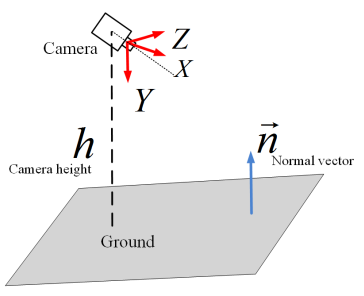
\includegraphics[width=.5\textwidth]{ground_plane}
	\caption{Camera attached at fixed height showing ground \cite{ground}}
	\label{fig:ground_plane}
\end{figure}
\begin{figure}[H]
	\centering
	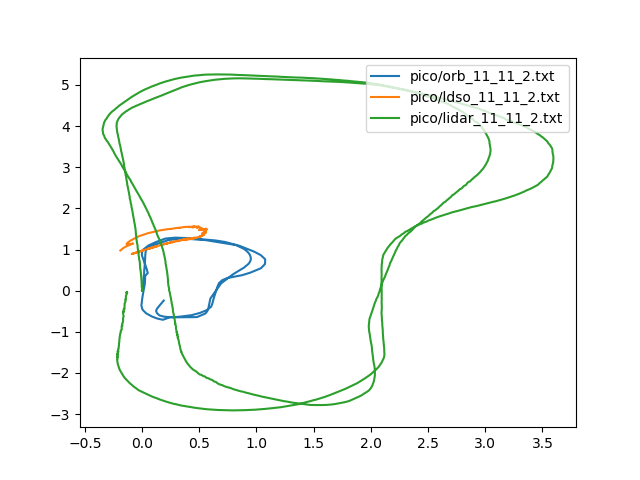
\includegraphics[width=1.0\textwidth]{orb_lidar}
	\caption{Scale comparison of \acrshort{orb}-\acrshort{slam} and \acrshort{ldso} with \acrshort{lidar} odometry}
	\label{fig:orb_lidar}
\end{figure}
\begin{figure}[H]
	\centering
	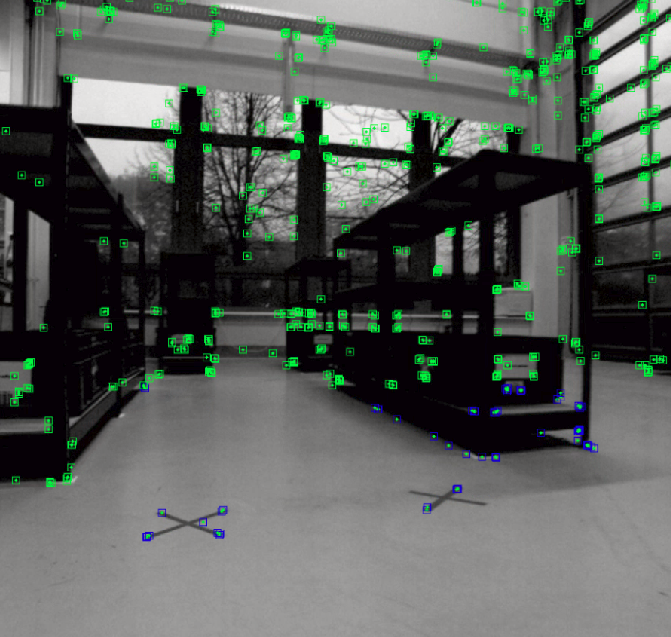
\includegraphics[width=0.6\textwidth]{ground_points}
	\caption{Ground points (blue rectangles) seen in one of the measurement}
	\label{fig:ground_points}
\end{figure}
\noindent Some features from \acrshort{roi} (ground plane) are detected and used into homography computation due to their planer behavior and initial camera height is then compared with actual one and finally absolute scale transfers to camera pose. A function is implemented based on that but the absolute scale cannot be retrieved because of insufficient and inconsistent features found on ground in neighboring frames and there are also some outliers which makes it even harder. Though an outlier removal is done using Opencv \textit{triangulatePoints} function, satisfactory result is not found as shown in figure \ref{fig:orb_lidar2}. The absolute scale comparison with \acrshort{lidar} odometry can be found in figure \ref{fig:orb_lidar3}.
\begin{figure}[H]
	\centering
	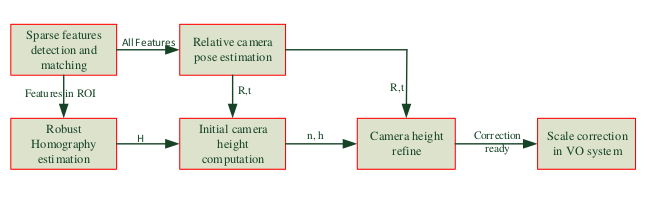
\includegraphics[width=1.0\linewidth]{scale_process}
	\caption{Absolute scale estimation procedure using camera height approach \cite{ground}}
	\label{fig:scale_process}
\end{figure}
\begin{figure}[H]
	\begin{subfigure}{.5\textwidth}
		\centering
		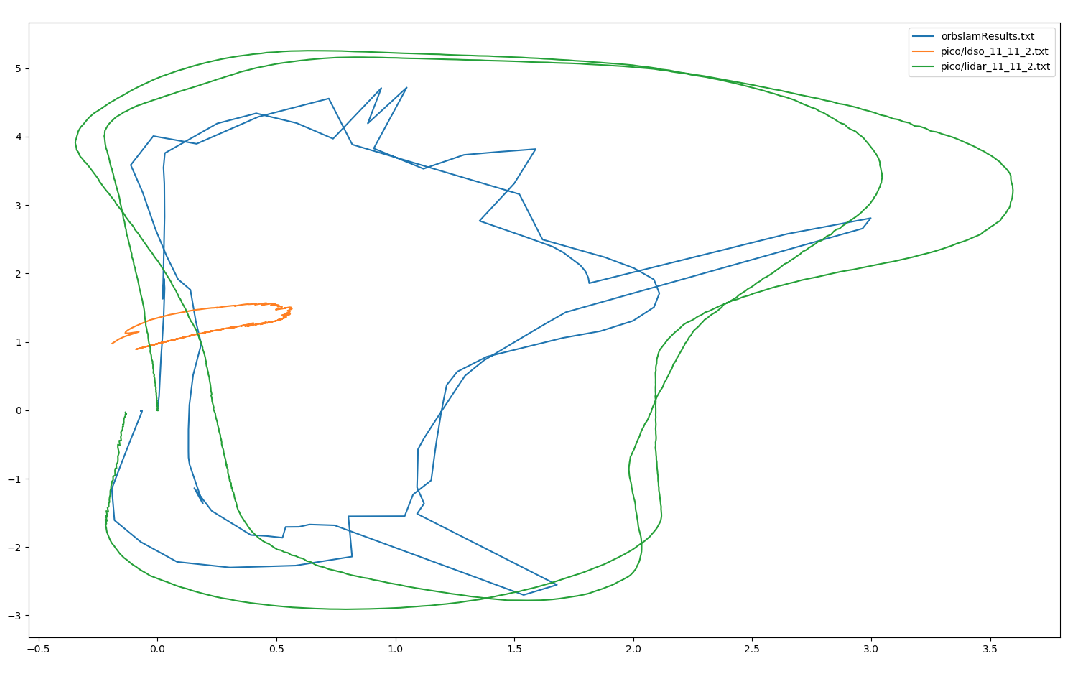
\includegraphics[width=1.0\linewidth]{orb_lidar2}
		\caption{Scale calculated using ground plane approach}
		\label{fig:orb_lidar2}
	\end{subfigure}%
	\begin{subfigure}{.5\textwidth}
		\centering
		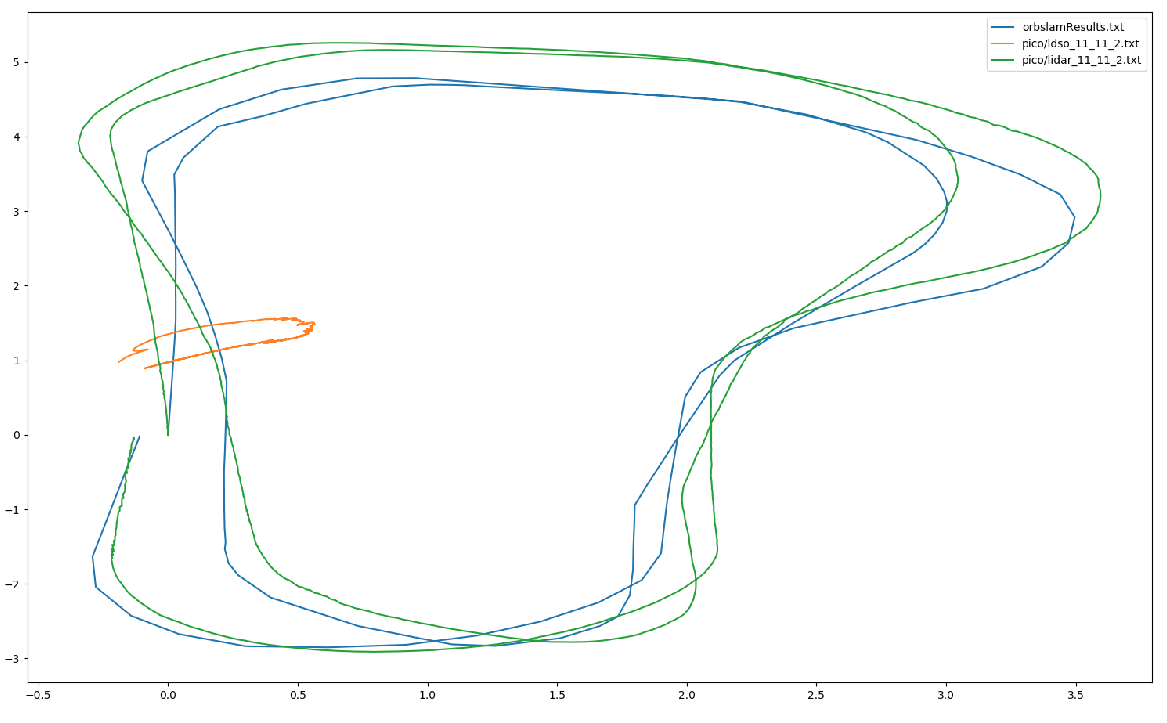
\includegraphics[width=1.0\linewidth]{orb_lidar3}
		\caption{Absolute scale comparison}
		\label{fig:orb_lidar3}
	\end{subfigure}
	\caption{Different scale comparison of \acrshort{orb}-\acrshort{slam} and \acrshort{lidar} odometry }
	\label{fig:plots}
\end{figure}

\subsection{\acrshort{ldso}}
\acrshort{ldso} has very complex implementation which restricts to modify the code but the parameters are mostly defined in one file \textit{settings.cc} which makes it easy to parameter tuning.
\begin{itemize} 
	\item The memory consumption was too high which made the algorithm interrupting in between. Some parameters like value of \textit{setting\_desiredPointDensity} and \textit{setting\_desiredImmatureDensity} are required to reduced.
 	\item To make initialization faster, \textit{setting\_outlierTH} value is increased from 144 to 225 to remove lesser outliers.
	\item In loop closing module for improve loop correction a dilated inverse depth map of 3 pixels is included around the active pixels. 
\end{itemize}